\documentclass[a4paper,11pt, twoside]{article}

%%%%%%%%%%%%%%%%%%%%%%%%%%%%%
%% Packages
% System - Sprache
\usepackage[utf8x]{inputenc}
\usepackage[ngerman]{babel}
\usepackage[T1]{fontenc}
\usepackage{lmodern}
\usepackage{ucs}
\PrerenderUnicode{äüößÄÜÖ} 

\usepackage[colorlinks=true, pdfborder={0 0 0}, pdftex, breaklinks=true, linkcolor=blue, citecolor=orange , filecolor=purple , urlcolor=purple, linktocpage=true]{hyperref}

% Seiten Layout
\usepackage{fancyhdr}
\usepackage[left=2cm,right=3cm,top=3cm,bottom=2.5cm]{geometry}

% TIKZ
\usepackage{tikz}
\usepackage{pgf}

% Inhalt
\usepackage{wrapfig} %floatfig
\usepackage{sidecap} %floatfig
\usepackage{float}
\usepackage{dpfloat}
\usepackage{algorithmicx}
\usepackage{algorithm}
\usepackage{algpseudocode}
\usepackage{prettyref}
\usepackage{titleref}
\usepackage{listings}
\usepackage{glossaries}
\usepackage{nomencl}
\usepackage{cite}
\usepackage{graphicx}
\usepackage{verbatim}
\usepackage[font=small,labelfont=bf]{caption}

% Mathe
\usepackage{calc}
\usepackage{ifthen}
\usepackage{times}
\usepackage{amsmath}
\usepackage{mathtools}

% hyperref
\usepackage[nohyperlinks%,printonlyused, 
]{acronym}

\newcommand\mpar[1]{\marginpar {\flushleft\small #1}}
\setlength{\marginparwidth}{2cm}

%%%%%%%%%%%%%%%%%%%%%%%%%%%%%
%% Farben
\definecolor{lightgrey}{gray}{.8}
\definecolor{lila}{rgb}{0.,0,0.5}

%%%%%%%%%%%%%%%%%%%%%%%%%%%%%
%% Farben
\definecolor{lightgrey}{gray}{.8}
\definecolor{lila}{rgb}{0.,0,0.5}

\begin{document}

\title{
\textbf{Kosten und Märkte}\\
Zusammenfassung
}

\author{Christian Silfang}
\date{Somersemester 2014}

\parskip1.5ex
\parindent0em

\pagestyle{empty}
\maketitle
\thispagestyle{empty}
\cleardoublepage

%\noindent\rule[1ex]{\textwidth}{1pt}

%\vspace{1cm}
\tableofcontents
\cleardoublepage

\pagestyle{fancy}
	\renewcommand{\sectionmark}[1]{\markboth{#1}{}}
	\fancyhf{}
	\fancyhead[EL]{\thesection { }\leftmark}
	\fancyhead[OR]{{ }\rightmark}
	\renewcommand{\headrulewidth}{0.4pt}
	\pagenumbering{arabic}
	
  \fancyfoot[EL]{\textbf{\thepage}}
	\fancyfoot[OR]{\textbf{\thepage}} 
	
	\setcounter{page}{1}

\section{Planung \& Kontrolle}

\subsection{Grundbegriffe}

\subsubsection*{Eigenschaften von Strategien}
\begin{itemize}
	\item legen Aktivitätsfelder fest, sind kokurrenzbezogen
	\item sind konkurrenzbezogen
	\item nehmen Bezug auf die Umweltsituation und –entwicklung (Chancen und Bedrohungen)
	\item beziehen sich auf Unternehmensressourcen relativ zur Konkurrenz
	\item zeigen Einstellungen/Wertvorstellungen der Entscheidungsträger
	\item auf gesamtes Geschäftsfeld ausgerichtet
	\item hohe Bedeutung für Vermögens-/Ertragslage des Unternehmens
	\item weitreichende Konsequenzen
	\item zukunftsorientiert
	\item können (!) einem systematischen Planungsprozeß entspringen
\end{itemize}

\subsubsection*{Leitfragen}
\begin{enumerate}
	\item Tätigkeit in welchen Geschäftsfeldern?
	\item Wie soll Wettbewerb in Geschäftsfeldern bestritten werden?
	\item Was ist die längerfristige Erfolgsbasis (Kernkompetenz)?
\end{enumerate}

\textbf{Gesamtunternehmen:} Gesamtunternehmensstrategie (Corporate Strategy)\\
\textbf{Geschäftsfeld:} Wettbewerbsstrategie (Business Strategy)

\subsection{Umweltanalyse}

Umweltanalyse ist Kernstück der strategischen Analyse und ermittelt Chancen/Bedrohungen

\subsubsection*{Betrachtungen}
$\rightarrow$ Wettbewerbsumfeld/Geschäftsfeld: Analyse der Branchenstruktur nach \footnote{
%% Fußnote
\textbf{Five-Forces von Porter}: Markterfolg hängt im wesentlichen von Marktstruktur ab (Seite 28/Abbildung):
\begin{enumerate}
	\item Wettbewerber einer Branche (Rivalen)
	\item Potenzielle neue Anbieter (Bedrohung)
	\item Ersatzprodukteb(Substitutionsgefahr)
	\item Lieferanten (Verhandlungsstärke)
	\item Abnehmer (Verhandlungsmacht)
\end{enumerate}
}{\textit{Porter}}

\texttt{GRAFIK}

$\rightarrow$ Betrachtet allgemeine Umwelt:
\begin{itemize}
	\item Makroökonomische Umwelt
	\begin{itemize}
		\item Konjunkturentwicklung, Wechselkurse, Entwicklung des Arbeitsmarktes, wirtschaftliche Entwicklung (global/nach Region)
	\end{itemize}
	\item Technologische Umwelt
	\begin{itemize}
		\item Entwicklung der Technologie als wesentlicher Treiber, S-Kurven-Modell (Technologielebenszyklus)
	\end{itemize}
	\item Politisch-rechtliche Umwelt
	\begin{itemize}
		\item politische Entwicklung auf allen Ebenen, Zölle/Subventionen
		\item internationale Tendenzen (Verschuldung, 3. Welt, Kyoto, Osteuropa), Krisen
	\end{itemize}
	\item Soziokulturelle Umwelt
	\begin{itemize}
		\item Demographische Entwicklung, Wertewandel
	\end{itemize}
	\item Natürliche Umwelt
	\begin{itemize}
		\item Benötigte Ressourcen (Reichweite/Verteilung), Entsorgung
	\end{itemize}
\end{itemize}

\subsubsection*{Vorgehensweise}
Bestimmung von relevanten Schlüsselgrößen und Prognosen über deren Entwicklung. Analyse von Querverbindungen über Entwurf/Bewertung von alternativen Szenarien. Festellung der Prämisse für weitere Planungsprozesse.

\subsection{Unternehmensanalyse}

Ermittlung der eigenen Stärken und Schwächen, dazu sind zwei Sichtweisen erforderlich:
\begin{enumerate}
	\item \textbf{Wertschöpfungssicht:} eigene Stärken/Schwähen relativ zur Konkurrenz
	\item \textbf{Kundensicht:} kritische Erfolgsfaktoren aus Sicht des Marktes, eigenes Profil vs. Profil der Wettbewerber
\end{enumerate}
$\rightarrow$ beide Sichtweisen ergeben \textbf{Potentiale und Wettbewerbsvorteile}(Vgl. Wertkette nach \textit{Porter})
	%% Randnotiz	
	\mpar{\textcolor{red}{Abschätzung der eigenen preislichen Lage auf dem Markt}}
\texttt{GRAFIK}

Erfolgsfaktoren können in verschiedene Faktoren eingeteilt werden:
\begin{itemize}
	\item Finanzielle
	\item Physische $\rightarrow$ häufiger Erfolgsfaktor
	\item Humane $\rightarrow$ häufiger Erfolgsfaktor
	%% Randnotiz	
	\mpar{\textcolor{red}{Monopolstellung bei vorhanden Ressourcen ist immer wertvoll!}}
	\item Organisatorische
	\item Technologische
	\item Finanzielle
\end{itemize}
%% Randnotiz	
\mpar{\textcolor{red}{Ressourcen die jeder hat, sind nicht wertvoll!}}

\subsubsection*{Merkmale "`strategischer"' Ressourcen}
\begin{itemize}
	\item Einmaligkeit: knappe Ressourcen, monopolähnlicher Zugang  
	\item Eingeschränkte Imitierbarkeit: Zusammenhänge schwer erkennbar, historisch gewachsene Ressourcen/Situationen, soziale Komplexität	
	\item Fehlende Substituierbarkeit: Ressourcen sind nicht durch andere ersetzbar
	\item Wert für die Strategie: Ressourcen müssen gewinnbringend zur Steigerung der Wettbewerbsfähigkeit verwendet werden können
\end{itemize}

\subsubsection*{Möglichkeiten zur Selbstreflektion}
%% Randnotiz	
\mpar{\textcolor{red}{Erhebungen durch Kundenbefragung ODER Vergleich mit Konkurrenz}}
\[ \left.
\begin{array}{l l}
\text{\textbf{S}} & \quad \text{trength}\\
\text{\textbf{W}} & \quad \text{eakness}\\
\text{\textbf{O}} & \quad \text{portunities}\\
\text{\textbf{T}} & \quad \text{reatments}
\end{array} 
\right\} \to \text{SWOT-Analyse} \quad \quad	\begin{array}{c|c}
					  	 S & W \\
					  	 \hline
					  	 O & T
						\end{array} \]

Teilweise Betrachtung aus Sicht des Kunden, dazu Ermittlung kritischer Erfolgsfaktoren wie Qualität, Service, Flexibilität, Termintreue und Preis.

\subsection{Strategische Optionen}

%% Randnotiz	
\mpar{\textcolor{red}{Nischenmarkt: schwierig, falls besetzt}}
Es existieren \underline{drei} zentrale Fragen zur Ermittlung der strategischen Optionen:
\begin{enumerate}
	\item Wo soll konkurriert werden? (Ort des Wettbewerbs)
	\item Wie soll konkurriert werden? (Regeln des Wettbewerbs: Rabatte, Preisnachlass)
	\item Mit welcher Stoßrichtung soll konkurriert werden? (Schwerpunkt des Wettbewerbs: Massen- oder Billigproduktion)
\end{enumerate}

%%%%%%%%%%%%%%%%%%%%%%%%%%%%%%%%%%%%%%%
%% Bild: Diversifikation
\begin{figure}[h]
 \begin{center}
   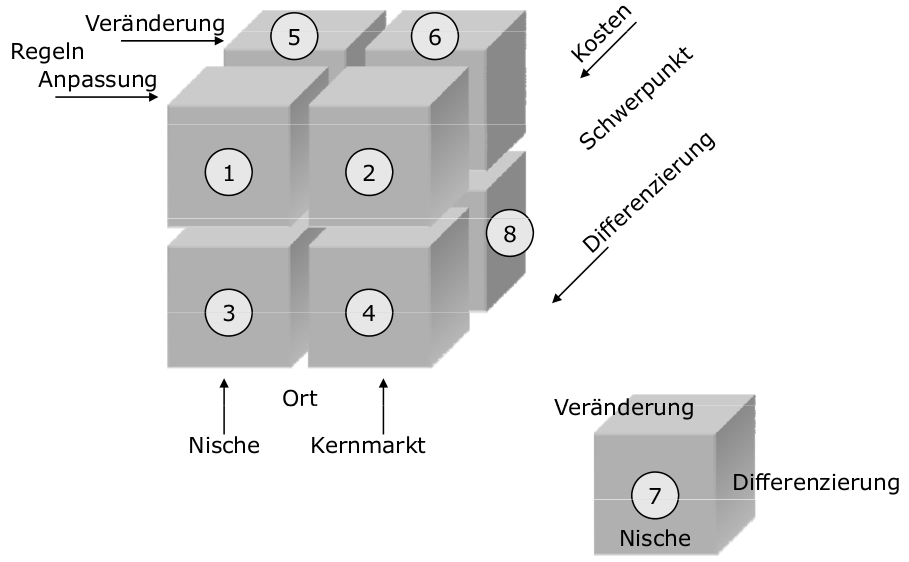
\includegraphics[scale=0.3]{bilder/strategische_optionen.png}
 \end{center}
\end{figure}
%%%%%%%%%%%%%%%%%%%%%%%%%%%%%%%%%%%%%%%

Überlegungen nur sinnvoll wenn Unternehmen in mehreren Geschäftsfeldern tätig ist oder eine Erweiterung auf mehrere geschäftsfelder geplant wird. 
Die möglichen Optionen sind:

\subsubsection*{Diversifikation} 
%%%%%%%%%%%%%%%%%%%%%%%%%%%%%%%%%%%%%%%
%% Bild: Diversifikation
\begin{figure}[h]
 \begin{center}
   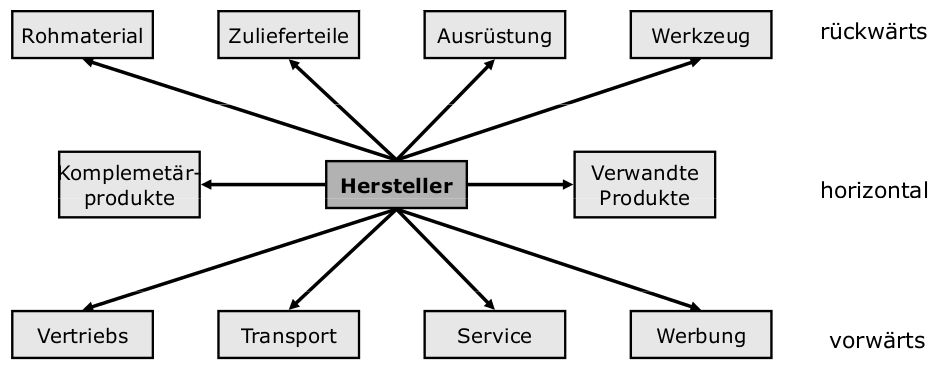
\includegraphics[scale=0.3]{bilder/diversifikation.png}
 \end{center}
\end{figure}
%%%%%%%%%%%%%%%%%%%%%%%%%%%%%%%%%%%%%%%
\newpage

\subsubsection*{Portfolio-Strategien} 

\textbf{?}: hohes Wachstum, aber relativ viel Konkurrenz\\
\textbf{$\star$}: großer Anteil und schnell wachsender Markt (bspw. Tablet-Produkte)\\
\textbf{Desinvestition}: schlecht, kein Wachstum und keine Anteile am Markt (Porter: "`nicht wachsender Markt"')\\ 
\textbf{Abschöpfung}: hoher Anteil, Wachstum stagniert ("`Milchkuh melken"')

%%%%%%%%%%%%%%%%%%%%%%%%%%%%%%%%%%%%%%%
%% Bild: Portfolio
\begin{figure}[h]
 \begin{center}
   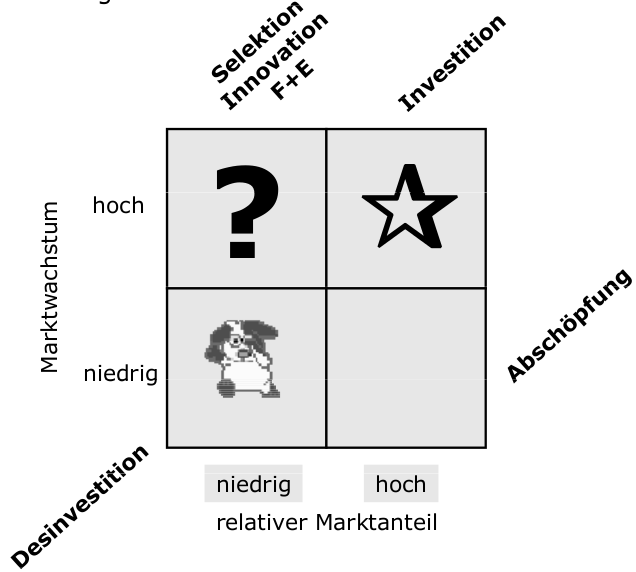
\includegraphics[scale=0.3]{bilder/portfolio.png}
 \end{center}
\end{figure}
%%%%%%%%%%%%%%%%%%%%%%%%%%%%%%%%%%%%%%%
\begin{center}
Alle 3 Diagramme müssen zueinander ins Verhältnis gebracht werden! $\downarrow$
\end{center}
%%%%%%%%%%%%%%%%%%%%%%%%%%%%%%%%%%%%%%%
%% Bild: Portfolio
\begin{figure}[h]
 \begin{center}
   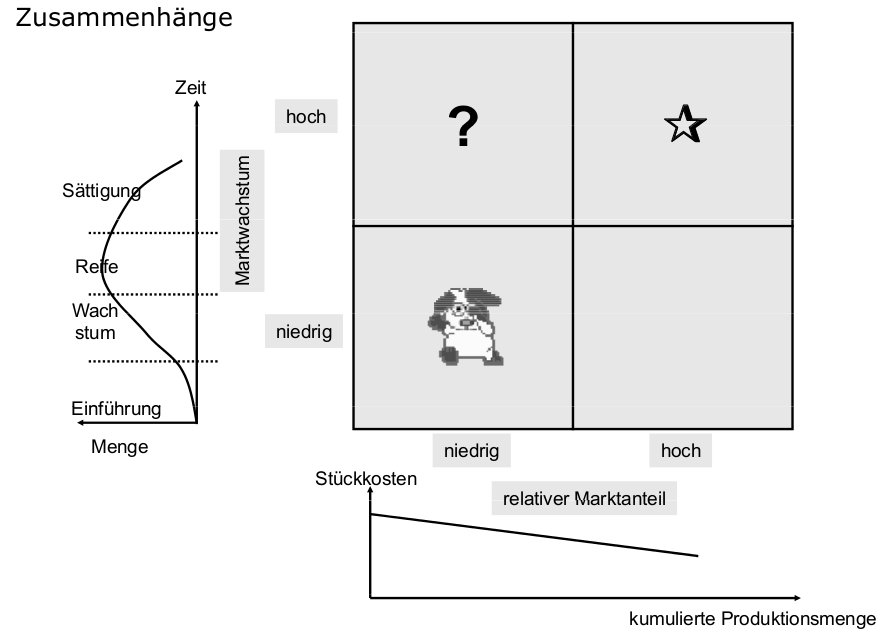
\includegraphics[scale=0.3]{bilder/portfolio_ext.png}
 \end{center}
\end{figure}
%%%%%%%%%%%%%%%%%%%%%%%%%%%%%%%%%%%%%%%

\subsubsection*{Internationalisierung} 
Ausdehnung der Geschäftstätigkeiten über Ländergrenzen hinweg, i.d.R. gleiche Produkt

National agierendes Unternehmen\\ 
\textit{Wie soll Markteintritt erfolgen?}
\begin{itemize}
	\item Export
	\item Lizenzvergabe oder Franchising
	\item Direktinvestition oder Akquisition
\end{itemize}

%% Randnotiz	
\mpar{\textcolor{red}{Steuern/Gesetzte nehmen Einfluss}}
International agierendes Unternehmen\\
\textit{Unterscheidung}\\
\begin{itemize}
	\item Globalisierung: das selbe Produkt und die selbe Wettbewerbsstrategie (diverse Ausführungen)
	\item Regionalisierung: Differenzierung des Produkts/Strategie
\end{itemize}

\subsubsection*{Kernkompetenzorientierung} 
Übergreifendes Qualifikationspotential, welches in verschiedenen Geschäftsfeldern den Aufbau von Wettbewerbsvorteilen ermöglicht

Merkmale von Kernkompetenzen:
\begin{itemize}
	\item Unternehmensweiter Geltungsbereich
	\item Dauerhafte Quelle von Wettbewerbsvorteilen
	\item historische Entwicklung
	\item kollektives Wissen
	\item Ressourcenwettbewerb
\end{itemize}
$\rightarrow$ Potentiale ausnutzen

\subsection{Strategische Wahl}
Auswahl der für das Unternehmen optimalen Strategie. Hierzu werden Beurteilungsgrößen herangezogen:
\begin{itemize}
	\item ökonomische Ziele
	\item Machbarkeit
	\item Akzeptanz
	\item ethische Vertretbarkeit
\end{itemize}
Dabei können verschiedene Probleme auftreten. Erfolge einer Strategie sind immer unsicher und ökonomische Auswirkungen immer nur schätzbar. Der "`Wert"' einer Strategie teilweise nicht quantifizierbar. Auswahlprozess ist komplex und nur teilweise rational.
 
\subsubsection*{Einflussfaktoren}

\texttt{GRAFIK}

\subsection{Strategieimplementation}
\underline{Drei} verschieden Punkte:

\subsubsection*{Strategische Maßnahmen}
\textit{"`structure follows strategy"'}\\
Kontingenztheorethischer Ausgangspunkt


\subsubsection*{Strategische Programme}
\textit{"`multidimensionale"' Zielsetzung}\\
Konkretisierung der Strategien in die einzelnen organisatorischen Bereiche und Ermittlung der kritischen Bereiche


\subsubsection*{Menschen/Führungssysteme}
\textit{"`strategy follows structure/personnel policy"'}\\
Strategische Personalplanung und -entwicklung sowie Problematik der Unternehmenskultur

$\rightarrow$ Balanced Scorecard

\texttt{GRAFIK + BEISPIEL}

\subsubsection*{Strategische Organisationsgestaltung}

\begin{tabular}{|l|l|}
\hline 
Einprodukt & Funktional/zentralisiert \\ 
\hline 
Verwandte Diversifikation & Divisional/dezentralisiert \\ 
\hline 
Konglomerate Diversifikation & Holding/stark dezentralisiert \\ 
\hline 
\end{tabular} 

Hat einen situativen Ansatz (Kontingent Ansatz). Bildung strategischer Geschäftseinheiten (SGE) in Anlehnung an die strategischen Geschäftsfelder. Mit Beachtung der Kernkompetenzen.

\subsubsection*{Strategische Personalpolitik}
Unterliegen Aspekten der Unternehmenskultur. Rückschlüsse der Personalentwicklung auf strategische Planung.

\subsection{Strategische Kontrolle}

\texttt{2 GRAFIKEN}

\subsection{Zusammenhänge der strategischen und operativen Planung}

\texttt{GRAFIK}

\newpage
\section{Absatz}

\subsection{Grundlagen}
Dient der Leistungsverwertung: Suche nach Abnehmern, Physische Distribution der Ware

x-Rs der Absatzwirtschaft:
\begin{itemize}
	\item richtige Ware
	\item richtige Menge
	\item richtige Qualität
	\item richtige Zeit
	\item richtiger Ort
\end{itemize}
$\rightarrow$ steigender Stellenwert des Absatzes

Minimale Fehlmengenkosten + Minimale Bestandskosten $\rightarrow$ Formel
\[
\text{Servicegrad} = \frac{\text{Anzahl der befriedigten Bedarfsanforderungen}}{\text{Anzahl aller Bedarfsanforderungen}} * 100\%
\]

\text{GRAFIK}

Erweiterung des Absatzbegriffs $\rightarrow$ Marketing\\ 
(= Konzeption der Unternehmensführung, die zur Erreichung der Unternehmensziele alle betrieblichen Aktivitäten konsequent auf die Erfordernisse des Absatzmarktes ausrichtet)

Aspekte des Marketings:
\begin{itemize}
	\item \textbf{Maxime}: Kunde als Ziel der Bemühungen
	\item  \textbf{Konzept}: geplanter und systematischer Einsatz der Instrumente zur Marktbeeinflussung und Gestaltung
	\item \textbf{Methode}: systematische Entscheidungsfindung und planmäßiges Vorgehen unter Einsatz wissenschaftlicher Methoden
\end{itemize}

Entwicklung von Merketingstrategien/Wachstumsstrategien 

\texttt{GRAFIK}

\textbf{Marktdurchdringung} (Abschöpfen des Marktpotentials)\\
...durch Erhöhung der Produktverwendung bei bestehenden Kunden\\
...durch Gewinnung von neuen Kunden\\
...durch Gewinnung von "`nicht"'-Verwendern\\

\textbf{Marktentwicklung} (Platzieren vorhandener Produkte in neuen Märkten)\\
Regionale Ausdehnung, neue Zielgruppen und Preisdifferenzierung

\textbf{Produktentwicklung} (Entwicklung neuer Produkte)\\
Innovationen und neue Produktvarianten

%% Randnotiz	
\mpar{\textcolor{red}{risikoreichste Wachstumstrategie}}

\textbf{Diversifikation} (Expansion in neue Geschäftsbereiche)\\
Horizontal: Erweiterung des Produktprogramms, mit ursprünglichem in sachlichem Zusammenhang\\
Vertikal: Vergrößerung der Tiefe des Produktprogramms (Vorwärtsintegration $\leftrightarrow$ Rückwärtsintegration)\\
Lateral: gänzlich neue Markt- und Produktgebiete (risikoreich)\\

\subsection{Marktforschung}
Beschaffung, Aufbereitung und Analyse von Informationen über Absatzmärkte zur Festlegung des optimalen Marketing-Mix

\textbf{Marketing-Mix}: (=optimale Abstimmung der Marketing-Instrumente zur Erreichnung der Ziele)\\
Produkt-. Preis-, Distributions- und Werbepolitik

\subsubsection*{Aufgaben}

\textbf{Analyse}
\begin{itemize}
	\item Erforschung der Grundstruktur des Marktes
	\item Zeitpunktbezogen 
\end{itemize}

\textbf{Beobachtung}
\begin{itemize}
	\item dynamische Komponente
	\item wesentliche Markteigenschaften (z.B. Konsolidierungen)
	\item A-Teile 
\end{itemize}

\textbf{Prognose}
\begin{itemize}
	\item Antizipation der zukünftigen Entwicklung wichtiger Trends (z.B. Substitutionsgüter)
	\item problematisch
\end{itemize}

\subsubsection*{Vorgehen}
1. Zieldefinition:\\
Zweck der Untersuchung, Art, Ausmaß und Qualität der zu beschaffenden Information

2. Wahl des Forschungsdesigns - Grundsätzlicher Aufbau der Studie:
\begin{itemize}
	\item Explorativ (Gewinnung qualitativer Daten als Basisinformation)
	%% Randnotiz	
\mpar{\textcolor{red}{Beispiel: "`Welche Eigenschaften muß eine Kaffeesorte für ältere Menschen aufweisen?"'}}
	\item Deskriptiv (Quantitative Beschreibung von Marktgegebenheiten, z.B. Absatzzahlen und Entwicklung des Marktanteils)
	\item Kausalanalytisch (Zusammenhänge zwischen Marktgegebenheiten, z.B. Wirkung der Verpackungsgestaltung auf den Marktanteil)
\end{itemize}

3. Informationsgewinnung - Wahl der Methode und des Umfangs der Untersuchung:\\
Primärforschung und Sekundärforschung

4. Auswertung der Information - Zielbezogene Analyse der erhobenen Daten:\\
Univariante Verfahren: Ermittlung einer Variablen (z.B. Kundenprofil eines Supermarkts)\\
Multivariante Verfahren: Ermittlung der Zusammenhänge mehrerer Variablen (z.B. Ladenöffnungszeiten und Eigenschaften der Käufergruppe)

5. Ableiten von Konsequenzen auf den Marketing-Mix

\subsubsection*{Methoden}

\texttt{GRAFIK}








\newpage
\section{Kosten- und Erfolgscontrolling}

\subsection{Grundlagen und Grundbegriffe}

\subsubsection*{Rechnungswesen}
Unterscheidung zwischen:
\begin{itemize}
	\item Externes Rechnungswesen: Finanz-, Geschäftsbuchhaltung, Jahresabschluss
	\item Internes Rechnungswesen Kosten- und Leistungsrechnung (interne Entscheidungsprozesse)
\end{itemize}

Aufgaben der Kosten- und Leistungsrechnung:\\
Erfassung anfallender Kosten und verursachungsgerechte Zurechnung der Kosten zu den Kostenträgern.

\subsection{Kostenartenrechnung}

\end{document} 
